\begin{center}
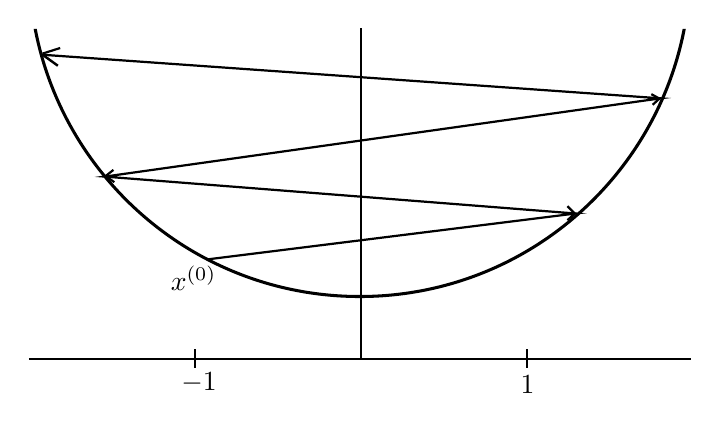
\begin{tikzpicture}[y=0.80pt, x=0.80pt, yscale=-1.000000, xscale=1.000000, inner sep=0pt, outer sep=0pt]
\begin{scope}[shift={(-0.53125,-802.625)}]
    \path[draw=black,line join=miter,line cap=butt,line width=0.832pt]
      (0.5406,951.8622) -- (299.4614,951.8622);
    \path[draw=black,line join=miter,line cap=butt,line width=0.588pt]
      (150.5199,952.1022) -- (150.5199,802.6222);
    \path[draw=black,line join=miter,line cap=butt,line width=0.965pt]
      (75.6030,947.4451) -- (75.6030,955.7591);
    \path[draw=black,line join=miter,line cap=butt,line width=0.965pt]
      (225.6030,947.4452) -- (225.6030,955.7592);
    \path[color=black,fill=black,line width=1.095pt] (2.7188,802.8438) .. controls
      (16.0212,872.0668) and (76.9019,924.3750) .. (150.0000,924.3750) .. controls
      (223.0981,924.3750) and (283.9788,872.0668) .. (297.2812,802.8438) --
      (295.8438,802.8438) .. controls (282.5683,871.3055) and (222.3498,923.0000) ..
      (150.0000,923.0000) .. controls (77.6419,923.0000) and (17.3964,871.3169) ..
      (4.1250,802.8438) -- (2.7188,802.8438) -- cycle;
    \path[draw=black,line join=miter,line cap=butt,line width=0.800pt]
      (81.3173,906.9002) -- (247.4874,886.1921) -- (34.8503,869.5246) --
      (285.8732,834.1692) -- (6.5660,814.4713);
    \path[draw=black,line join=miter,line cap=butt,line width=0.794pt]
      (6.7446,813.9662) -- (14.7009,811.4408);
    \path[draw=black,line join=miter,line cap=butt,line width=0.876pt]
      (6.6189,814.3739) -- (13.6578,819.4576);
    \path[draw=black,line join=miter,line cap=butt,line width=0.800pt]
      (282.3376,837.0734) -- (285.3681,834.2955) -- (281.7063,832.2752);
    \path[draw=black,line join=miter,line cap=butt,line width=0.800pt]
      (38.7646,866.4941) -- (35.2291,869.2720) -- (39.1434,872.0499);
    \path[draw=black,line join=miter,line cap=butt,line width=0.800pt]
      (243.8256,889.2225) -- (247.1086,886.1921) -- (243.8256,882.9091);
    \path[fill=black] (64.6498,921.0424) node[above right] (text3136) {$x^{(0)}$};
    \path[fill=black] (69.4141,967.3622) node[above right] (text3140) {$-1$};
    \path[fill=black] (222.6816,967.3622) node[above right] (text3140-7) {$1$};
\end{scope}
\end{tikzpicture}
\end{center}
